% $Id: client.tex 4644 2007-02-22 16:23:30Z mike $
% Local Variables:
% ispell-check-comments: nil
% Local IspellDict: american
% End:
% --------------------------------------------------------
% User documentation
% copyright by BREDEX GmbH 2004
% --------------------------------------------------------
\index{Client}
\index{Test Step}
\index{Test Case}
\index{Test Suite}
\index{Project}
\index{Workspace}
\index{Component}
\index{Action}
\index{Parameter}
\index{CAP}

The client is the interface with which the user interacts, where 
\gdsteps{}, \gdcases{}, \gdsuites and \gdprojects are created to test the 
application under test (\gdaut{}) 
(see \bxfigref{pyramide} and \bxfigref{testcasesandsteps}). 

\begin{figure}[h]
\begin{center}
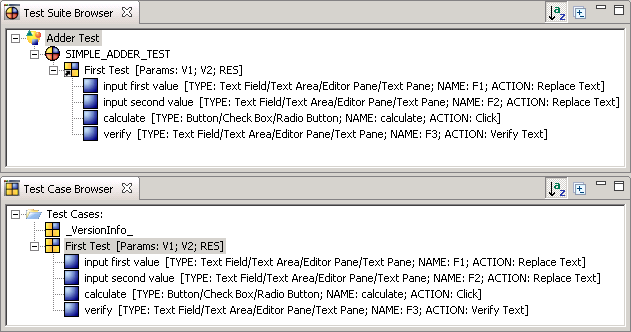
\includegraphics{GettingStarted/Structure/PS/testcasesandsteps}
\caption{\gdtestsuitebrowser and \gdtestcasebrowser containing a \gdcase}
\label{testcasesandsteps}
\end{center}
\end{figure}
\begin{description}
\item[\gdsteps]{ are the smallest 
entity in \GD{},  and consist of three elements:
\begin{itemize}
\item A user interface \textbf{C}omponent
\item An \textbf{A}ction to be performed on the component
\item \textbf{P}arameters for the Action.

In the program, these elements are referred to as \bxcaption{CAP}.
\end{itemize}}


\item[\gdcases]{ may contain
 any number of  \gdsteps and other \gdcases and are
displayed as a tree structure, comparable to a directory structure.}

\item[\gdsuites]{ may contain any
 number of \gdcases to be executed and are linked to an \gdaut{}. }

\item[\gdprojects]{may contain several \gdsuites{}.}
\end{description}

\subsubsection{Workspace}
Personal settings  are stored in a \bxcaption{workspace}. 
The default workspace is set up
 during installation, but a new path may be chosen when \GD starts. 

The default workspace can be changed using the Configuration Tool, which is 
located in the \gd installation directory, in the \bxcaption{configuration} folder. 

For information on the Configuration Tool, consult the Installation Manual. 
\bxcomment{AI}{Do we need to say anything about creating a Workspace?}
\bxcomment{AI}{Grafik?}
